% Dynamic Programming Part 2 -- Metropolis beamer slides
% Compile: pdflatex dynamic-programming-2.tex (x2)
\documentclass[10pt,aspectratio=169]{beamer}

\usetheme{metropolis}
\metroset{block=fill, numbering=fraction, progressbar=frametitle}

\usepackage[T1]{fontenc}
\usepackage{amsmath, amssymb}
\usepackage{listings}
\usepackage{booktabs}
\usepackage{tikz}
\usepackage{pgfplots}
\pgfplotsset{compat=1.18}
\usetikzlibrary{arrows.meta, positioning, decorations.pathreplacing, calc, matrix}

% ---- colors -------------------------------------------------------------
\definecolor{mLightBlue}{HTML}{4C72B0}
\definecolor{mGreen}{HTML}{55A868}
\definecolor{mRed}{HTML}{C44E52}
\definecolor{mGray}{HTML}{BFBFBF}
\setbeamercolor{alerted text}{fg=mRed}

% ---- code style ---------------------------------------------------------
\lstdefinestyle{jl}{
  basicstyle=\ttfamily\footnotesize,
  keywordstyle=\color{mRed}\bfseries,
  commentstyle=\color{mGreen}\itshape,
  numberstyle=\tiny\color{mGray},
  showstringspaces=false,
  breaklines=true,
  columns=fullflexible,
  morekeywords={function,for,in,if,else,elseif,end,return,length,while,using}
}
\lstset{style=jl}

% ---- title --------------------------------------------------------------
\title{Dynamic Programming, Part 2}
\subtitle{LCS, Knapsack, Weighted Interval Scheduling}
\date{}
\author{}

\begin{document}

\maketitle

% =========================================================================
\section{Longest Common Subsequence}

\begin{frame}{Subsequence, not Substring}
  A \alert{subsequence} deletes characters without reordering the rest.
  A \alert{substring} must be contiguous.

  \bigskip
  \begin{center}
  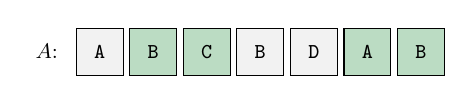
\begin{tikzpicture}[scale=0.85, every node/.style={transform shape}]
    \foreach \v/\fillc [count=\i from 0] in
      {A/black!5, B/mGreen!40, C/mGreen!40, B/black!5, D/black!5, A/mGreen!40, B/mGreen!40} {
      \node[draw, minimum size=7mm, fill=\fillc] at (\i*0.8,0) {\small \tt \v};
    }
    \node[left] at (-0.5,0) {\small $A$:};
  \end{tikzpicture}
  \end{center}

  \bigskip
  \begin{center}
    \small \texttt{BCAB} is a subsequence of \texttt{ABCBDAB}, but not a substring.
  \end{center}
\end{frame}

\begin{frame}{The Problem}
  Given $A[1 \ldots n]$ and $B[1 \ldots m]$, find the longest sequence that is a
  subsequence of \alert{both}.

  \bigskip
  \begin{center}
  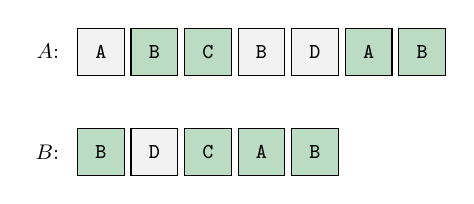
\begin{tikzpicture}[scale=0.85, every node/.style={transform shape}]
    \node[left] at (-0.5,0.9) {\small $A$:};
    \foreach \v/\fillc [count=\i from 0] in
      {A/black!5, B/mGreen!40, C/mGreen!40, B/black!5, D/black!5, A/mGreen!40, B/mGreen!40} {
      \node[draw, minimum size=7mm, fill=\fillc] at (\i*0.8,0.9) {\small \tt \v};
    }
    \node[left] at (-0.5,-0.6) {\small $B$:};
    \foreach \v/\fillc [count=\i from 0] in
      {B/mGreen!40, D/black!5, C/mGreen!40, A/mGreen!40, B/mGreen!40} {
      \node[draw, minimum size=7mm, fill=\fillc] at (\i*0.8,-0.6) {\small \tt \v};
    }
  \end{tikzpicture}
  \end{center}

  \bigskip
  \begin{center}
    \texttt{BCAB} has length $4$. \quad So does \texttt{BDAB}.\\
    \smallskip
    \small The LCS need not be unique.
  \end{center}
\end{frame}

\begin{frame}{The Table}
  \begin{block}{Definition}
    $LCS[i,j]$ = length of the LCS of $A[1 \ldots i]$ and $B[1 \ldots j]$.
  \end{block}

  \bigskip
  Look at the last characters. Two cases.

  \bigskip
  \begin{center}
  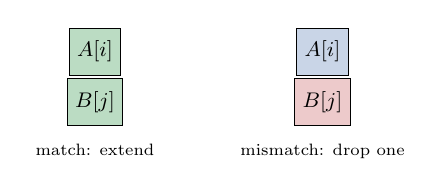
\begin{tikzpicture}[scale=0.85, every node/.style={transform shape},
      bx/.style={draw, minimum size=7mm}]
    \node[bx, fill=mGreen!40] at (0,0.75)  {\small $A[i]$};
    \node[bx, fill=mGreen!40] at (0,0)     {\small $B[j]$};
    \node[below] at (0,-0.5) {\scriptsize match: extend};
    \node[bx, fill=mLightBlue!30] at (3.4,0.75) {\small $A[i]$};
    \node[bx, fill=mRed!30]       at (3.4,0)    {\small $B[j]$};
    \node[below] at (3.4,-0.5) {\scriptsize mismatch: drop one};
  \end{tikzpicture}
  \end{center}
\end{frame}

\begin{frame}{The Recurrence}
  \begin{itemize}
    \item \textbf{$A[i] = B[j]$:} match them and extend, giving $LCS[i-1,j-1] + 1$.
    \pause
    \item \textbf{$A[i] \ne B[j]$:} the LCS cannot end with both, so drop one of
          them and take the better option.
  \end{itemize}

  \pause
  \bigskip
  \begin{alertblock}{}
    \[
      LCS[i,j] = \begin{cases}
        LCS[i-1,j-1] + 1 & \text{if } A[i] = B[j], \\[0.3em]
        \max\big( LCS[i-1,j],\; LCS[i,j-1] \big) & \text{otherwise.}
      \end{cases}
    \]
  \end{alertblock}

  \bigskip
  Base cases: $LCS[i,0] = 0$ and $LCS[0,j] = 0$.
\end{frame}

\begin{frame}{A Worked Table}
  $A = \texttt{ABCB}$, \quad $B = \texttt{BCB}$.

  \begin{center}
  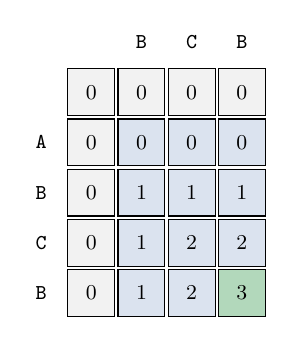
\begin{tikzpicture}[scale=0.85, every node/.style={transform shape},
      c/.style={draw, minimum size=7mm, font=\small}]
    % column headers
    \foreach \h [count=\j from 1] in {B,C,B}
      \node at (\j*0.75+0.75, 0.75) {\small \tt \h};
    % row headers
    \foreach \h [count=\i from 1] in {A,B,C,B}
      \node at (0, -\i*0.75) {\small \tt \h};
    % row 0
    \foreach \j in {0,...,3} \node[c, fill=black!5] at (\j*0.75+0.75, 0) {0};
    % body
    \foreach \row [count=\i from 1] in {{0,0,0},{1,1,1},{1,2,2},{1,2,3}} {
      \node[c, fill=black!5] at (0.75, -\i*0.75) {0};
      \foreach \v [count=\j from 1] in \row {
        \ifnum\i=4 \ifnum\j=3 \def\fc{mGreen!45}\else\def\fc{mLightBlue!20}\fi
        \else \def\fc{mLightBlue!20}\fi
        \node[c, fill=\fc] at (\j*0.75+0.75, -\i*0.75) {\v};
      }
    }
  \end{tikzpicture}
  \end{center}

  \begin{center}
    $LCS[4,3] = 3$, achieved by \texttt{BCB}.
  \end{center}
\end{frame}

\begin{frame}[fragile]{Implementation: Filling the Table}
  Row by row, left to right.

  \begin{lstlisting}
function lcs(A::String, B::String)
    n, m = length(A), length(B)
    L = OffsetArray(zeros(Int, n + 1, m + 1), 0:n, 0:m)

    for i in 1:n
        for j in 1:m
            if A[i] == B[j]
                L[i, j] = L[i - 1, j - 1] + 1
            else
                L[i, j] = max(L[i - 1, j], L[i, j - 1])
            end
        end
    end

    # continued on the next slide
  \end{lstlisting}
\end{frame}

\begin{frame}[fragile]{Implementation: Recovering the String}
  Walk back from $(n,m)$, prepending a character on every match.

  \begin{lstlisting}
    # ... still inside lcs(A, B)

    lcs_str = ""
    i, j = n, m
    while i > 0 && j > 0
        if A[i] == B[j]
            lcs_str = string(A[i]) * lcs_str
            i -= 1; j -= 1
        elseif L[i - 1, j] > L[i, j - 1]
            i -= 1
        else
            j -= 1
        end
    end

    return L[n, m], lcs_str
end
  \end{lstlisting}
\end{frame}

% =========================================================================
\section{0/1 Knapsack: Maximize Value}

\begin{frame}{The Problem}
  $n$ items, item $i$ has weight $w[i]$ and value $v[i]$. Knapsack capacity $W$.
  Each item is taken \alert{whole or not at all}.

  \bigskip
  \begin{center}
  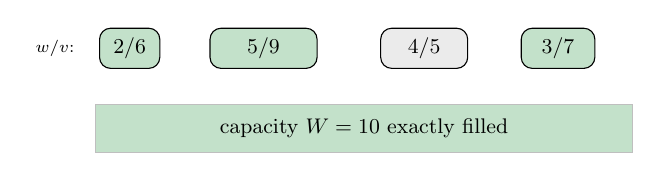
\begin{tikzpicture}[scale=0.85, every node/.style={transform shape},
      it/.style={draw, rounded corners, minimum height=6mm, font=\small}]
    \node[it, fill=mGreen!35, minimum width=9mm]  (a) at (0,0)   {$2 / 6$};
    \node[it, fill=mGreen!35, minimum width=16mm] (b) at (2.0,0) {$5 / 9$};
    \node[it, fill=black!8,   minimum width=13mm] (c) at (4.4,0) {$4 / 5$};
    \node[it, fill=mGreen!35, minimum width=11mm] (d) at (6.4,0) {$3 / 7$};
    \node[left] at (-0.7,0) {\scriptsize $w/v$:};
    \draw[mGray, thick] (-0.5,-0.85) rectangle (7.5,-1.55);
    \fill[mGreen!35] (-0.5,-0.85) rectangle (7.5,-1.55);
    \node at (3.5,-1.2) {\small capacity $W = 10$ exactly filled};
  \end{tikzpicture}
  \end{center}

  \bigskip
  \begin{center}
    Items $1, 2, 4$: weight $2+5+3 = 10$, value $6+9+7 = \alert{22}$.
  \end{center}
\end{frame}

\begin{frame}{Greedy Fails}
  Sorting by value-to-weight ratio is tempting, but wrong.

  \bigskip
  \begin{center}
    $W = 40$, \quad items $(20,100)$, $(20,100)$, $(25,150)$.
  \end{center}

  \bigskip
  \begin{center}
  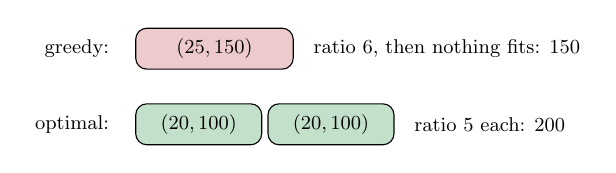
\begin{tikzpicture}[scale=0.8, every node/.style={transform shape},
      it/.style={draw, rounded corners, minimum height=6.5mm, font=\small}]
    % greedy
    \node[left] at (-0.3,0.55) {\small greedy:};
    \node[it, fill=mRed!30, minimum width=25mm] at (1.25,0.55) {$(25,150)$};
    \node[right] at (2.7,0.55) {\small ratio $6$, then nothing fits: \alert{150}};
    % optimal
    \node[left] at (-0.3,-0.65) {\small optimal:};
    \node[it, fill=mGreen!35, minimum width=20mm] at (1.0,-0.65) {$(20,100)$};
    \node[it, fill=mGreen!35, minimum width=20mm] at (3.1,-0.65) {$(20,100)$};
    \node[right] at (4.3,-0.65) {\small ratio $5$ each: \alert{200}};
  \end{tikzpicture}
  \end{center}
\end{frame}

\begin{frame}{The Table}
  \begin{block}{Definition}
    $K[i,c]$ = maximum value using items $1 \ldots i$ with capacity $c$.
  \end{block}

  \bigskip
  For item $i$ at capacity $c$:

  \begin{itemize}
    \item \textbf{Skip it:} capacity unchanged, value $K[i-1, c]$.
    \pause
    \item \textbf{Take it:} only if $w[i] \le c$; spend $w[i]$, gain $v[i]$,
          giving $K[i-1, c - w[i]] + v[i]$.
  \end{itemize}

  \pause
  \bigskip
  \begin{alertblock}{}
    \[
      K[i,c] = \begin{cases}
        K[i-1,c] & \text{if } w[i] > c, \\[0.3em]
        \max\big( K[i-1,c],\; K[i-1, c-w[i]] + v[i] \big) & \text{otherwise.}
      \end{cases}
    \]
  \end{alertblock}
\end{frame}

\begin{frame}{Filling the Table}
  Base cases: $K[0,c] = 0$ and $K[i,0] = 0$.

  \bigskip
  \begin{center}
  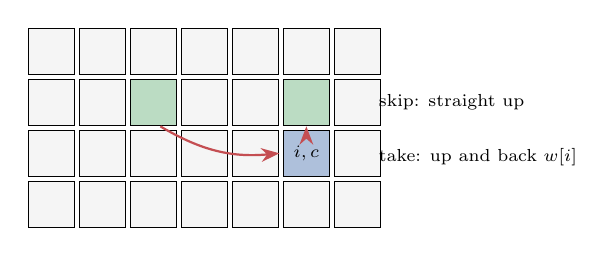
\begin{tikzpicture}[scale=0.9, every node/.style={transform shape},
      c/.style={draw, minimum size=6.5mm}]
    \foreach \i in {0,...,3} \foreach \j in {0,...,6} {
      \node[c, fill=black!4] at (\j*0.72, -\i*0.72) {};
    }
    \node[c, fill=mLightBlue!45] at (0.72*5, -0.72*2) {\scriptsize $i,c$};
    \node[c, fill=mGreen!40]     at (0.72*5, -0.72*1) {};
    \node[c, fill=mGreen!40]     at (0.72*2, -0.72*1) {};
    \draw[-{Stealth}, mRed, thick] (0.72*5, -0.72*1-0.38) -- (0.72*5, -0.72*2+0.38);
    \draw[-{Stealth}, mRed, thick] (0.72*2+0.1, -0.72*1-0.34) to[bend right=18] (0.72*5-0.38, -0.72*2);
    \node[right] at (4.5,-0.72) {\scriptsize skip: straight up};
    \node[right] at (4.5,-1.5)  {\scriptsize take: up and back $w[i]$};
  \end{tikzpicture}
  \end{center}

  \bigskip
  \begin{center}
    Row $i$ reads only row $i-1$, so fill row by row. Answer at $K[n, W]$.\\
    \smallskip
    Running time $O(nW)$.
  \end{center}
\end{frame}

\begin{frame}[fragile]{Implementation}
  \begin{lstlisting}[basicstyle=\ttfamily\scriptsize]
function knapsack(weights, values, W)
    n = length(weights)
    K = OffsetArray(zeros(Int, n + 1, W + 1), 0:n, 0:W)

    for i in 1:n
        for c in 0:W
            K[i, c] = K[i - 1, c]                 # skip item i
            if weights[i] <= c
                K[i, c] = max(K[i, c],
                    K[i - 1, c - weights[i]] + values[i])   # take item i
            end
        end
    end

    selected_items = []               # trace back
    c = W
    for i in n:-1:1
        if K[i, c] != K[i - 1, c]     # value changed, so item i was taken
            push!(selected_items, i)
            c -= weights[i]
        end
    end

    return K[n, W], selected_items
end
  \end{lstlisting}
\end{frame}

% =========================================================================
\section{0/1 Knapsack: Minimize Weight}

\begin{frame}{Flip the Table Around}
  Index by \alert{value} instead of capacity. Let
  $V_{\max} = \sum_{i=1}^{n} v[i]$.

  \bigskip
  \begin{block}{Definition}
    $M[i,u]$ = minimum weight to achieve \alert{exactly} value $u$
    using items $1 \ldots i$, or $+\infty$ if impossible.
  \end{block}

  \bigskip
  \begin{center}
    \small This version pays off later, when we approximate knapsack in time
    independent of $W$.
  \end{center}
\end{frame}

\begin{frame}{The Recurrence}
  For item $i$ at target value $u$:

  \begin{itemize}
    \item \textbf{Skip it:} $M[i-1, u]$.
    \pause
    \item \textbf{Take it:} only if $v[i] \le u$; add weight $w[i]$ and ask the
          rest for value $u - v[i]$, giving $M[i-1, u - v[i]] + w[i]$.
  \end{itemize}

  \pause
  \bigskip
  \begin{alertblock}{}
    \[
      M[i,u] = \begin{cases}
        M[i-1,u] & \text{if } v[i] > u, \\[0.3em]
        \min\big( M[i-1,u],\; M[i-1, u-v[i]] + w[i] \big) & \text{otherwise.}
      \end{cases}
    \]
  \end{alertblock}

  \bigskip
  Base cases: $M[0,0] = 0$, and $M[0,u] = +\infty$ for $u > 0$.
\end{frame}

\begin{frame}{Reading Off the Answer}
  The table gives minimum weight per value. We want the best value that
  \alert{fits}.

  \bigskip
  \begin{center}
  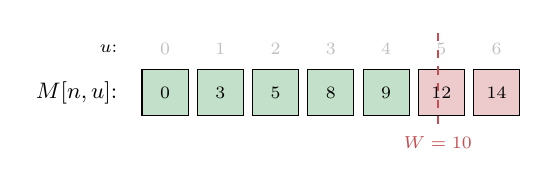
\begin{tikzpicture}[scale=0.9, every node/.style={transform shape},
      c/.style={draw, minimum size=6.5mm, font=\scriptsize}]
    \foreach \v/\fillc [count=\j from 0] in
      {0/mGreen!35, 3/mGreen!35, 5/mGreen!35, 8/mGreen!35, 9/mGreen!35,
       12/mRed!30, 14/mRed!30} {
      \node[c, fill=\fillc] at (\j*0.78,0) {\v};
      \node[mGray] at (\j*0.78,0.62) {\scriptsize $\the\numexpr\j\relax$};
    }
    \node[left] at (-0.55,0)    {\small $M[n,u]$:};
    \node[left] at (-0.55,0.62) {\scriptsize $u$:};
    \draw[mRed, thick, dashed] (3.85,-0.45) -- (3.85,0.9);
    \node[below, mRed] at (3.85,-0.5) {\scriptsize $W = 10$};
  \end{tikzpicture}
  \end{center}

  \bigskip
  \begin{center}
    Scan $u$ from $0$ to $V_{\max}$ and keep the largest with $M[n,u] \le W$.\\
    \smallskip
    Here the answer is $u = 4$.
  \end{center}

  \bigskip
  \begin{center}
    Running time $O(n \cdot V_{\max})$.
  \end{center}
\end{frame}

\begin{frame}[fragile]{Implementation}
  \begin{lstlisting}[basicstyle=\ttfamily\scriptsize]
function knapsack_weight(weights, values, W)
    n = length(weights)
    V_max = sum(values)
    INF = typemax(Int) div 2                  # div 2 avoids overflow
    M = OffsetArray(fill(INF, n + 1, V_max + 1), 0:n, 0:V_max)
    M[0, 0] = 0

    for i in 1:n
        for u in 0:V_max
            M[i, u] = M[i - 1, u]             # skip item i
            if values[i] <= u && M[i - 1, u - values[i]] < INF
                M[i, u] = min(M[i, u],
                    M[i - 1, u - values[i]] + weights[i])  # take item i
            end
        end
    end

    best = 0                                  # largest value that fits
    for u in 0:V_max
        if M[n, u] <= W
            best = u
        end
    end

    return best
end
  \end{lstlisting}
\end{frame}

\begin{frame}{Exercise}
  \begin{enumerate}
    \item Modify \texttt{knapsack\_weight} to also return \emph{which} items are
          selected, like the traceback in the value-based version.
    \bigskip
    \item Both versions take each item at most once. What changes if an item may
          be taken \alert{any number of times}?
  \end{enumerate}

  \bigskip
  \begin{center}
    \small The second one is the \emph{unbounded} knapsack problem.
  \end{center}
\end{frame}

\begin{frame}{Solution 1}
  Same trick as before: compare against the skip case.

  \bigskip
  Walk back from $(n, u^{*})$ where $u^{*}$ is the answer. At row $i$:

  \begin{itemize}
    \item If $M[i,u] = M[i-1,u]$, item $i$ was skipped. Move to $(i-1, u)$.
    \item Otherwise item $i$ was taken. Record it and move to $(i-1,\, u - v[i])$.
  \end{itemize}

  \bigskip
  \begin{center}
    \small The walk touches one cell per row, so it costs $O(n)$.
  \end{center}
\end{frame}

\begin{frame}{Solution 2}
  If item $i$ can be reused, then after taking it we may take it \alert{again}.
  So the second term looks at row $i$, not row $i-1$:

  \bigskip
  \begin{alertblock}{}
    \[
      K[i,c] = \max\big( K[i-1,c],\; \underbrace{K[i,\, c-w[i]]}_{\text{row } i} + v[i] \big)
    \]
  \end{alertblock}

  \bigskip
  \begin{center}
  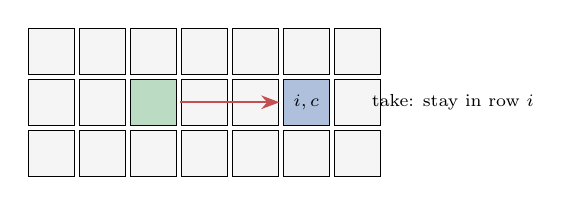
\begin{tikzpicture}[scale=0.9, every node/.style={transform shape},
      c/.style={draw, minimum size=6.5mm}]
    \foreach \i in {0,...,2} \foreach \j in {0,...,6} {
      \node[c, fill=black!4] at (\j*0.72, -\i*0.72) {};
    }
    \node[c, fill=mLightBlue!45] at (0.72*5, -0.72*1) {\scriptsize $i,c$};
    \node[c, fill=mGreen!40]     at (0.72*2, -0.72*1) {};
    \draw[-{Stealth}, mRed, thick] (0.72*2+0.38, -0.72*1) -- (0.72*5-0.38, -0.72*1);
    \node[right] at (4.4,-0.72) {\scriptsize take: stay in row $i$};
  \end{tikzpicture}
  \end{center}

  \bigskip
  \begin{center}
    \small One dimension collapses: $K[c] = \max_i \big( K[c - w[i]] + v[i] \big)$.
  \end{center}
\end{frame}

% =========================================================================
\section{Weighted Interval Scheduling}

\begin{frame}{The Problem}
  $n$ jobs, job $i$ has start $s[i]$, finish $f[i]$, and weight $v[i] > 0$.
  Two jobs are \alert{compatible} if they do not overlap.

  \bigskip
  \begin{center}
  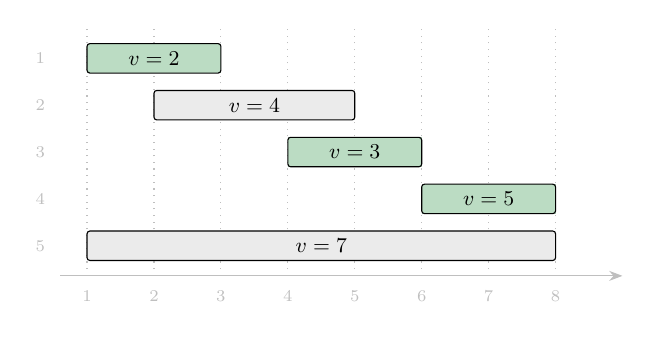
\begin{tikzpicture}[scale=0.85, every node/.style={transform shape},
      bar/.style={draw, rounded corners=1pt}]
    \foreach \t in {1,...,8} \draw[mGray, dotted] (\t,-3.25) -- (\t,0.45);
    \draw[-{Stealth}, mGray] (0.6,-3.25) -- (9.0,-3.25);
    \foreach \t in {1,...,8} \node[mGray] at (\t,-3.55) {\scriptsize \t};
    % job / start / finish / row / fill
    \foreach \id/\st/\fin/\y/\fc/\vv in {
        1/1/3/0/mGreen!40/2, 2/2/5/-0.7/black!8/4, 3/4/6/-1.4/mGreen!40/3,
        4/6/8/-2.1/mGreen!40/5, 5/1/8/-2.8/black!8/7} {
      \fill[\fc] (\st,\y-0.22) rectangle (\fin,\y+0.22);
      \draw[bar] (\st,\y-0.22) rectangle (\fin,\y+0.22);
      \node at ({(\st+\fin)/2},\y) {\small $v=\vv$};
      \node[mGray] at (0.3,\y) {\scriptsize \id};
    }
  \end{tikzpicture}
  \end{center}

  \bigskip
  \begin{center}
    Jobs $1, 3, 4$ are compatible with total weight $\alert{10}$, beating job
    $5$ alone at $7$.
  \end{center}
\end{frame}

\begin{frame}{Preprocessing}
  Sort the jobs by finish time: $f[1] \le f[2] \le \cdots \le f[n]$.

  \bigskip
  \begin{block}{Definition}
    $p[i]$ = the largest $j < i$ with $f[j] \le s[i]$, \; or $0$ if none exists.
  \end{block}

  \bigskip
  In words: the \alert{latest job that finishes before job $i$ starts}.

  \bigskip
  \begin{center}
  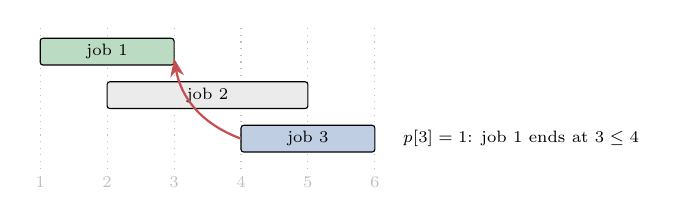
\begin{tikzpicture}[scale=0.85, every node/.style={transform shape},
      bar/.style={draw, rounded corners=1pt}]
    \foreach \t in {1,...,6} \draw[mGray, dotted] (\t,-1.75) -- (\t,0.35);
    \foreach \t in {1,...,6} \node[mGray] at (\t,-1.95) {\scriptsize \t};
    \foreach \id/\st/\fin/\y/\fc in {
        1/1/3/0/mGreen!40, 2/2/5/-0.65/black!8, 3/4/6/-1.3/mLightBlue!35} {
      \fill[\fc] (\st,\y-0.2) rectangle (\fin,\y+0.2);
      \draw[bar] (\st,\y-0.2) rectangle (\fin,\y+0.2);
      \node at ({(\st+\fin)/2},\y) {\scriptsize job \id};
    }
    \draw[-{Stealth}, mRed, thick] (4,-1.3) to[bend left=30] (3,-0.1);
    \node[right] at (6.3,-1.3) {\scriptsize $p[3] = 1$: job $1$ ends at $3 \le 4$};
  \end{tikzpicture}
  \end{center}

  \bigskip
  \begin{center}
    \small Computable in $O(n \log n)$ by binary search after sorting.
  \end{center}
\end{frame}

\begin{frame}{The Recurrence}
  For job $i$:

  \begin{itemize}
    \item \textbf{Skip it:} the best among the first $i-1$ jobs, $dp[i-1]$.
    \pause
    \item \textbf{Take it:} gain $v[i]$, then the best among jobs compatible with
          $i$, which is exactly $dp[p[i]]$.
  \end{itemize}

  \pause
  \bigskip
  \begin{alertblock}{}
    \[
      dp[i] = \max\big( dp[i-1],\; v[i] + dp[p[i]] \big)
    \]
  \end{alertblock}

  \bigskip
  Base case $dp[0] = 0$. Fill $dp[1], \ldots, dp[n]$ in order.

  \bigskip
  \begin{center}
    \small $p[i]$ is what makes this work: it skips over every incompatible job
    at once.
  \end{center}
\end{frame}

\begin{frame}{Working the Example}
  \begin{center}
  \begin{tabular}{lcccccc}
    \toprule
    $i$      & 0 & 1 & 2 & 3 & 4 & 5 \\
    \midrule
    $v[i]$   &   & 2 & 4 & 3 & 5 & 7 \\
    $p[i]$   &   & 0 & 0 & 1 & 3 & 0 \\
    \midrule
    $dp[i]$  & 0 & 2 & 4 & 5 & \alert{10} & 10 \\
    \bottomrule
  \end{tabular}
  \end{center}

  \bigskip
  \begin{itemize}
    \item $dp[3] = \max(dp[2],\; 3 + dp[1]) = \max(4, 5) = 5$.
    \item $dp[4] = \max(dp[3],\; 5 + dp[3]) = \max(5, 10) = 10$.
    \item $dp[5] = \max(dp[4],\; 7 + dp[0]) = \max(10, 7) = 10$.
  \end{itemize}

  \bigskip
  \begin{center}
    Answer $10$, from jobs $\{1, 3, 4\}$.
  \end{center}
\end{frame}

\begin{frame}[fragile]{Implementation: Preprocessing}
  Sort by finish time, then find each $p[i]$ by binary search.

  \begin{lstlisting}[basicstyle=\ttfamily\scriptsize]
function weighted_interval_scheduling(starts, finishes, weights)
    n = length(starts)

    order = sortperm(finishes)        # sort by finish time
    s, f, v = starts[order], finishes[order], weights[order]

    p = zeros(Int, n)                 # p[i] by binary search
    for i in 1:n
        lo, hi = 1, i - 1
        while lo <= hi
            mid = (lo + hi) div 2
            if f[mid] <= s[i]
                p[i] = mid; lo = mid + 1
            else
                hi = mid - 1
            end
        end
    end

    # continued on the next slide
  \end{lstlisting}
\end{frame}

\begin{frame}[fragile]{Implementation: Table and Traceback}
  \begin{lstlisting}[basicstyle=\ttfamily\scriptsize]
    # ... still inside weighted_interval_scheduling

    dp = OffsetArray(zeros(Int, n + 1), 0:n)
    for i in 1:n
        dp[i] = max(dp[i - 1], v[i] + dp[p[i]])
    end

    selected = Int[]                  # trace back
    i = n
    while i >= 1
        if v[i] + dp[p[i]] > dp[i - 1]
            push!(selected, order[i])  # job i was taken
            i = p[i]                   # jump over conflicts
        else
            i -= 1
        end
    end

    return dp[n], sort(selected)
end
  \end{lstlisting}
\end{frame}

\begin{frame}{Running Time and Traceback}
  \begin{itemize}
    \item Sorting: $O(n \log n)$.
    \item Computing every $p[i]$ by binary search: $O(n \log n)$.
    \item Filling the table: $O(n)$.
  \end{itemize}

  \bigskip
  \begin{alertblock}{}
    \[
      O(n \log n)
    \]
  \end{alertblock}

  \bigskip
  To recover the jobs, walk back from $i = n$:
  if $v[i] + dp[p[i]] > dp[i-1]$, job $i$ was taken, so record it and jump to
  $p[i]$; otherwise move to $i-1$.
\end{frame}

\end{document}
